\documentclass{article}

%%% Fill details here (in the second brackets)
\newcommand{\name}{Kaushik Dutta and Sung Min Ha}     % Your name (First Last)
\newcommand{\wustlkey}{CSE515T 2021 Final Project Report}             % Your WUSTL Key
%%%



%%%%%%%%%%%%%%%%%%%%%% Formatting Stuff %%%%%%%%%%%%%%%%%%%%%%%%%%%
\usepackage{times}
\usepackage[T1]{fontenc}


\setlength{\parskip}{1em}\setlength{\parindent}{0pt}
\linespread{1.25}
\usepackage[margin=0.7in,top=1in]{geometry}\usepackage{fancyhdr}
\pagestyle{fancy}\lhead{\bf \name}\rhead{\bf \wustlkey}\cfoot{\thepage}
\newcommand{\info}{\clearpage \subsection*{Information}}
\newcommand{\solution}[1]{\clearpage \subsection*{Solution #1}}
\newcommand{\spart}[1]{\paragraph{(#1)}}
%%%%%%%%%%%%%%%%%%%%%%%%%%%%%%%%%%%%%%%%%%%%%%%%%%%%%%%%%%%%%%%%%%%


%%% Add any more packages if you want to
\usepackage{amsmath,graphicx}
\usepackage{hyperref}
\usepackage{multirow}
%\usepackage{biblatex}
\usepackage[english]{babel}
\usepackage[backend=biber,style=alphabetic,sorting=ynt]{biblatex}
\addbibresource{ref.bib}

\title{Predicting English Premier League match results using Bayesian Hierarchical Model}

\begin{document}

\maketitle

\section{Introduction}
The statistical modelling of sports data has become increasingly popular in the last few years after the advent of machine learning which gives the ability to construct predictive models with unprecedented accuracy. For ages the betting companies have employed statistical intuition based on the team’s performance to calculate odds for predicting football results. But the biggest challenge in accurately predicting the results of a football match are the uncertainty pertaining to the results and thus it cannot be realized by a linear model. The football results prediction is based on complex non linear parameters encompassing a team’s performance over a varying timeframe and depending on a wide range of factors ranging from player performance statistics to home field advantage. To accommodate the non-linearity of the data, we propose a Bayesian Hierarchical Model that can be employed to predict the ranking of the English Premier League season alongwith a prediction of results and scores of a particular match in the season. A major reason behind choosing English Premier League is because it is highly competitive in nature and there is a high incidence of upsets (where weak teams outscore strong teams). The world was awed when the football club Leicester City won the championship in 2016, against all odds, but this demonstrates the highly unpredictable nature of the game, and therefore the difficulty of the problem we are trying to tackle.

\section{Method}

\subsection{Dataset and Preprocessing}
For this project we considered the English Premier League 2017-2018 season data. The English Premier League is the first division football league of the UK contested by 20 teams where each team plays against each other twice ( home and away ). A total of 380 matches are played in a season and the team with the highest point is declared winner. The top four teams of the league table goes on to play UEFA Champions League. The next three teams qualify for the Europa League and the bottom three teams are relegated to the Second Division league. We obtained our dataset from \url{http://www.football-data.co.uk/data.php}. The dataset has match statistics for all the matches in the season in terms of goals scored, corners, shots , fouls , red and yellow cards for both home and away teams. For preprocessing we trimmed the dataset to only include features which directly or indirectly affects the final match results and arranged the matches in a longitudinal fashion according to their dates.

\subsection{Feature Selection and Feature Engineering}
The quality of results in the prediction task is directly associated to the quality of the feature set used for modelling the system hence choosing the right features is of paramount importance. We divided the available features into two categories : 1) Attack and Defence Parameters consisting of the feature like goals scored and full/half time results which directly affect the match results and 2) Indirect Features consisting of the feature like corners, fouls, shots etc which provides us with mathematical insights regarding team performance and influence the match result in an indirect way. 
    When designing our model’s features for the prediction of football results, we wanted to introduce features that could provide us with useful quantifiable insights for judging the recent performance of a team. To this end we engineered two unique features called Form and Streak. These features enhance the predictive power of the model by incorporating the fact that recent performance of the team has the ability to influence the current game. The mathematical formulation for the engineered features are given as :

\subsubsection{Streak}
This feature encapsulates the recent improving/declining trend in the performance of a team. The Streak value for a team is computed by assigning a score to each match result and taking the mean of the previous k scores, where k is a hyper-parameter. We also included a temporal dimension to the Streak feature by placing time-dependent weights on the scores of the previous games of a team, obtaining a feature that we refer to as the Weighted Streak (greater weights for recent games, decreasing gradually for non-recent games).

\begin{equation}
\delta_j = \Sigma_{p=j-k}^{j-1} \frac{2(p-(j-k-1) res_{p}}{3k(k+1)}
\label{eq:streak}
\end{equation}

where, $\delta_j$ is the Weighted Streak of a team in the $j$-th match and the resp is point each team gets as per the result of the match (0-Loss, 1-Draw , 3-Win)

\subsubsection{Form}
This feature encapsulates the recent performance of the team relative to its opponents. The Form value of each team is initialized to one at the beginning of each season and then updated after each match according to the result of the match i.e. win,draw,loss. Our mathematical formulation of Form ensures that a greater coefficient update is provided if a weak team triumphs over a strong team, and vice-versa. In the case of a draw, the Form of a weak team increases while that of a strong team decreases. 
When a team $\alpha$ beats $\beta$ we can write the Form ($\xi$) equation for the teams as:
\begin{equation}
\xi_{j}^{\alpha}= \xi_{j-1}^{\alpha}  + \gamma\xi_{j-1}^{\beta}
\label{eq:form_1}
\end{equation}

\begin{equation}
\xi_{j}^{\beta}= \xi_{j-1}^{\beta}  - \gamma\xi_{j-1}^{\beta}
\label{eq:form_2}
\end{equation}

where $\gamma$ is the stealing fraction signifying the weight to be added/subtracted in case of win/loss

\subsubsection{Model Description}

The Poisson Distribution is widely acceptable as a modelling approach for the distribution of the number of goals involving two competing teams. In this problem we are assuming two conditionally independent Poisson variables for the number of goals scored, correlation is taken into account, since the observable variables are mixed at an upper level. Moreover, as we are framed in a Bayesian context, prediction of a new game under the model is naturally accommodated by means of the posterior predictive distribution. As discussed the league is played by N = 20 teams and the number of goals scored by the home and the away team in gth game (g = 1,2,3,…,380) of the season given by yg1 and yg2. The observed count vector is y = ($y_{g1} , y_{g2}$), which are independent Poisson random variables given by Eqn. 1. The parameters $\theta = (\theta_{g1} , \theta_{g2})$ gives the scoring intensity in the gth game of the season and j = 1 for home team and j = 2 for away team.

\begin{equation}
y_{g(j)} | \theta_{g(j)} = Poisson(\theta_{g(j)}
\label{eq:y_theta}
\end{equation}

We model the scoring intensity parameters as a log linear random effect model based on the work of Karlis and Ntzoufras (2003) \cite{karlis_ntzoufras_2003} and is given by the following two equations \ref{eq:log_g1} and \ref{eq:log_g2} for the home and away.


\begin{equation}
log \theta_{g1} = home + att_{h(g)} + def_{a(g)} + intercept
\label{eq:log_g1}
\end{equation}

\begin{equation}
log \theta_{g2} = att_{a(g)} + def_{h(g)} + intercept
\label{eq:log_g2}
\end{equation}

The home parameter represents the advantage of the home team playing in favorable conditions and is designed to be a constant distribution for all teams across the season. The other two parameters are the att and def  i.e. the attack and defense ability of the team. The goaling intensity of a team is calculated by the addition of its attacking ability and the opponents defensive ability. The attack and defense ability parameters are computed by the cumulative effect of the following parameters i.e. number of goals, shots and shots on target, corners, fouls, red and yellow cards, form and streak for both home and away team.

\begin{equation}
att_g = att_{goals} + att_{shots} + att_{shots-target} + att_{corners} - att_{fouls} - att_{yellow-card} - att_{red-card} + att_{streak} +att_{form}
\label{eq:att}
\end{equation}

\begin{equation}
def_g = def_{goals} + def_{shots} + def_{shots-target} + def_{corners} - def_{fouls} - def_{yellow-card} - def_{red-card} + def_{streak} +def_{form}
\label{eq:def}
\end{equation}

The attacking and defensive parameters are positively affected by goals, shots, corners, streak and form while they are negatively impacted by fouls and red/yellow cards (hence they are subtracted from the net attack and defense ability of the team). Now that we have the model parameters ready we have to specify some suitable prior distributions for the random parameters. The home parameter is modelled as a fixed effect, hence it is assumed as flat standard prior Normal Distribution given in Eqn. \ref{eq:home}. The attack and defence ability are modelled separately for each parameters for each teams T = (1,2,....,20) with a normal distribution having mean $\mu_{att}$ and variance $\tau_{att}$ and given in Eqn. \ref{eq:att_dist}.

\begin{equation}
home \sim Normal(0, 0001)
\label{eq:home_dist}
\end{equation}

\begin{equation}
att_t \sim Normal(\mu_{att}, \tau_{att})
\label{eq:att_dist}
\end{equation}

\begin{equation}
def_t \sim Normal(\mu_{def}, \tau_{def})
\label{eq:def_dist}
\end{equation}

As suggested by the works of Karlis and Ntzoufras (2003) we need to impose some identifiability constraints on the team-specific parameters hence we use sum-to-zero constraints for all the parameters used to compute attacking and defensive ability i.e. $\Sigma_{t=1}^{T} att_{t} = \Sigma_{t=1}^{T} def_{t}=1$. Finally, the hyper-priors of the attack and defense effects are modelled independently using again flat prior distributions given by Eqn. \ref{eq:mu_att_dist} to \ref{eq:tau_def_dist}.

\begin{equation}
\mu_{att} \sim Normal(0, 0.0001)
\label{eq:mu_att_dist}
\end{equation}

\begin{equation}
\mu_{def} \sim Normal(0, 0.0001)
\label{eq:mu_def_dist}
\end{equation}

\begin{equation}
\tau_{att} \sim Gamma(0.1, 0.1)
\label{eq:tau_att_dist}
\end{equation}

\begin{equation}
\tau_{def} \sim Gamma(0.1, 0.1)
\label{eq:tau_def_dist}
\end{equation}

\begin{figure*}[!htb]
\centering
\includegraphics[width=40em]{Final_Report_Figures/Hierarchical_Model.png}
\caption{The Representation of the Hierarchical Model}
\label{fig:hierarchical_model}
\end{figure*}

The inherent hierarchical nature of the model kind of implies that there is an effect on the observed variable vector y due to the latent unobservable hyperparameters $\eta= (att, def , att , def)$ . In fact, the components of $\eta$ represent a latent structure that we assume to be common for all the games played in a season and that determine the average scoring rate. Each game contributes to the estimation of these parameters, which in turn generate the main effects that explain the variations in the parameters $\theta$ and therefore implying a form of correlation on the observed counts y. 

\section{Results}

\begin{figure*}[!htb]
\centering
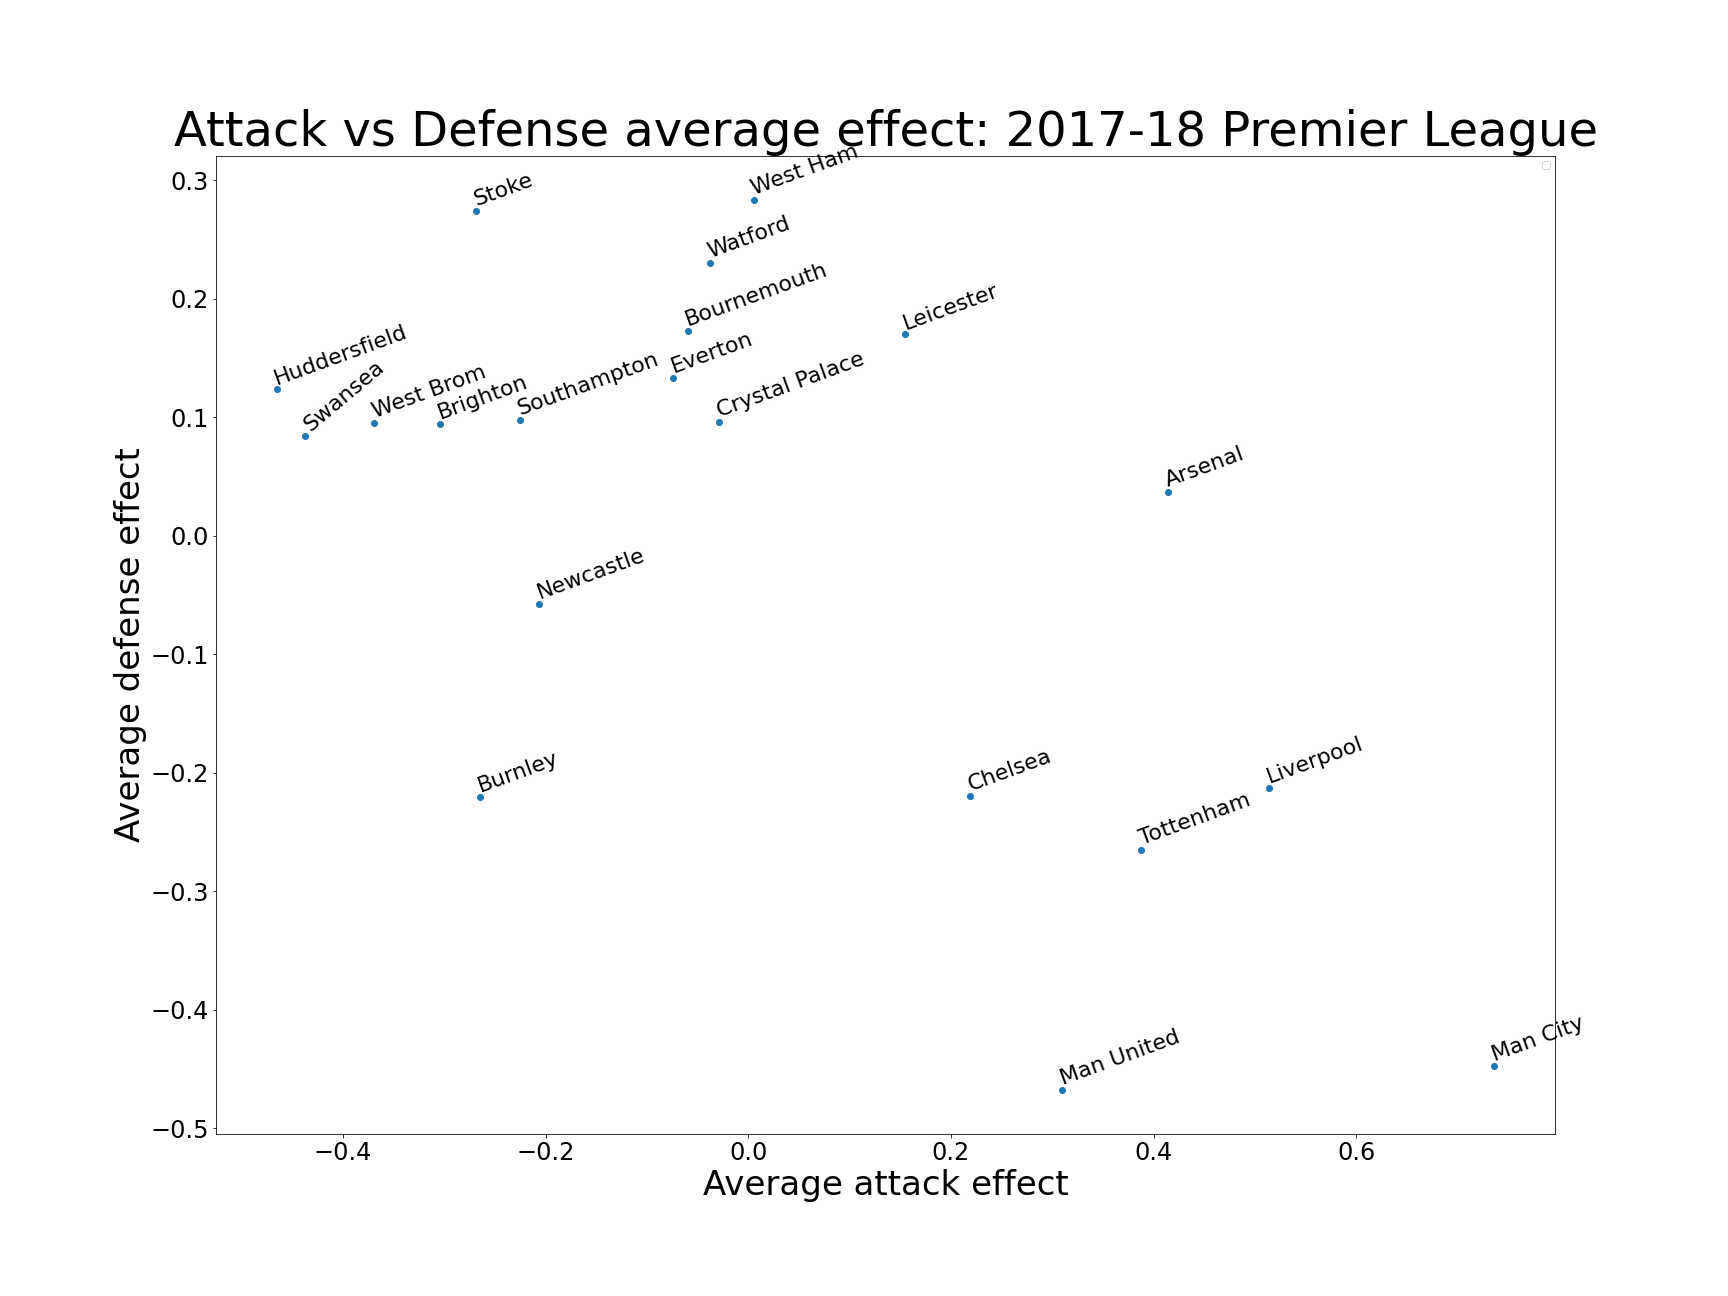
\includegraphics[width=40em]{Final_Report_Figures/scatter_avg_att_avg_def_20000_4000_20.png}
\caption{Attacking Ability VS Defensive Ability average effect for each team}
\label{fig:att_def_scatterplot}
\end{figure*}

According to the Bayesian approach the objective of our modelling is two-fold: first we wish to estimate the values of the attack and defence abilities of each team through which we can explain the scoring rate. This task is accomplished by the entering evidence observed in the goal scored vector (y) i.e. the likelihood and updating the prior distributions by a Markov Chain Monte Carlo (MCMC) procedure.  Table 1 summarizes statistics for the posterior distributions of the coefficients for the log-linear model describing the scoring intensity and the average attacking and defensive ability for each team is depicted in Fig. 2. We observe that the top four teams of that season ( Man City, Liverpool, Man United, Tottenham ) have higher posterior value for att and lower posterior value for def parameter. Man City the league champion for that year has the highest posterior for attack and the lowest posterior for defence. We also observe that for the bottom three teams i.e. Swansea, West Brom and Stoke have higher defensive posterior and lower attacking posterior suggesting they have more tendency to accede goals than scoring them. We also assumed that there is an inherent advantage for a team playing at home conditions and it is validated by the positive posterior mean for the home parameter of 0.284 (95\% CI, 0.169-0.401). We also considered an intercept parameter to give a uniform weightage to all the teams and also for the evaluation of away team scoring propensity. It also has a positive posterior mean of 0.037 (95\% CI, -0.063 - 0.136 ) signifying the away team factor also has some effect though not as dominant as the home team factor (Table 2). Furthermore, using equation 2 and 3, where atth(g)and defa(g)are zero-centered and home and intercept are constant values over a season and across all teams, we note that on average, the difference between home team score and away team score is predicted as ehome+intercept+0-eintercept+00.3408. With the actual data, we observed the average home score of 1.53 and away score of 1.15, for an observed difference in scores of 0.38 goals. We note from the similar value of predicted difference to actual difference in home and away scores that the model accurately estimated the home team advantage.

% Please add the following required packages to your document preamble:
% \usepackage{multirow}
\begin{table}[!htb]
\centering
\begin{tabular}{c|cccc|cccc}
\multirow{2}{*}{Team} & \multicolumn{4}{c|}{Attack}               & \multicolumn{4}{c}{Defense}               \\
                      & mean     & 2.50\%   & median   & 97.50\%  & mean     & 2.50\%   & median   & 97.50\%  \\ \hline
Arsenal               & 0.16588  & -0.2695  & 0.171398 & 0.500935 & -0.03586 & -0.27504 & -0.05564 & 0.217835 \\
Brighton              & -0.08838 & -0.43944 & -0.09538 & 0.356826 & 0.186183 & -0.2253  & 0.1795   & 0.53247  \\
Chelsea               & 0.017751 & -0.42171 & 0.026327 & 0.388936 & -0.10574 & -0.55694 & -0.10015 & 0.266319 \\
Crystal Palace        & 0.160214 & -0.04913 & 0.151332 & 0.395689 & 0.049696 & -0.28228 & 0.019035 & 0.385244 \\
Everton               & -0.07619 & -0.52102 & -0.02499 & 0.230095 & 0.021921 & -0.3693  & 0.018135 & 0.424184 \\
Southampton           & -0.09361 & -0.53298 & -0.06786 & 0.269567 & -0.01088 & -0.26426 & -0.01972 & 0.304954 \\
Watford               & 0.133206 & -0.32008 & 0.141774 & 0.537631 & 0.078818 & -0.27905 & 0.068123 & 0.476231 \\
West Brom             & -0.16773 & -0.57494 & -0.1472  & 0.142359 & 0.048288 & -0.24153 & 0.062213 & 0.356659 \\
Man United            & 0.157401 & -0.22843 & 0.150232 & 0.583509 & -0.20889 & -0.6698  & -0.20234 & 0.169697 \\
Newcastle             & -0.15355 & -0.5521  & -0.15651 & 0.235987 & 0.000329 & -0.23298 & 0.012996 & 0.225301 \\
Bournemouth           & -0.11214 & -0.37054 & -0.10584 & 0.116302 & 0.07689  & -0.24199 & 0.06963  & 0.474801 \\
Burnley               & -0.1398  & -0.57079 & -0.12747 & 0.297614 & -0.06604 & -0.45223 & -0.05894 & 0.257646 \\
Leicester             & 0.101308 & -0.18645 & 0.092653 & 0.437958 & 0.079157 & -0.28793 & 0.072431 & 0.471868 \\
Liverpool             & 0.178749 & -0.2033  & 0.154364 & 0.579239 & -0.10165 & -0.48196 & -0.09993 & 0.258778 \\
Stoke                 & -0.12206 & -0.45943 & -0.10613 & 0.259741 & 0.149268 & -0.20383 & 0.151795 & 0.504233 \\
Swansea               & -0.17799 & -0.67315 & -0.14613 & 0.314619 & -0.03705 & -0.42407 & -0.01273 & 0.256929 \\
Huddersfield          & -0.17887 & -0.63874 & -0.1614  & 0.314923 & 0.070606 & -0.24724 & 0.072733 & 0.400955 \\
Tottenham             & 0.123119 & -0.23711 & 0.111466 & 0.593627 & -0.12543 & -0.52889 & -0.11792 & 0.178844 \\
Man City              & 0.304239 & -0.06582 & 0.294613 & 0.715463 & -0.17417 & -0.62358 & -0.16807 & 0.248987 \\
West Ham              & -0.03154 & -0.13414 & -0.02919 & 0.077529 & 0.10457  & -0.25399 & 0.101079 & 0.460631
\end{tabular}
\caption{\label{tab:att_def_stats}Statistical Estimates on Attack and Defense Effects of the Model}
\end{table}

\begin{table}[!htb]
\centering
\begin{tabular}{c|cccc}
          & \textbf{mean} & \textbf{2.50\%} & \textbf{median} & \textbf{97.50\%} \\ \hline
Home      & 0.284818805   & 0.169524643     & 0.28921925      & 0.40125784       \\
Intercept & 0.03767081    & -0.063000434    & 0.039115445     & 0.136080733     
\end{tabular}
\caption{\label{tab:home_intercept_stats}Statistical Estimates on Home and Intercept Effects of the Model}
\end{table}

The second and probably more interesting objective of the model is that of prediction of the match results. We can use the results derived in the implied posterior distributions for the vector $\theta$ to predict a future occurrence of a similar game. To that end, we produced a vector of 1000 replications for the posterior predictive distribution of y that we used for the purpose of model checking. From the 1000 model simulations we take the median and the 95\% CI for each team and is depicted in Fig. 3. We can observe from Fig. 4 that for most of the teams the Bayesian model produces a good fit to the observed results. There are some disparities in prediction as we can observe from Fig 3. and Supplementary Fig. 1 and Supplementary Fig. 2 for the higher and lower performing team due to overshrinkage. Due to this effect all parameters have the tendency to be pulled towards their group mean, hence top performing teams have lower predicted goals/points whereas bottom performing teams have higher predicted goals/points. Contextually, the top performing and bottom performing teams may have large deviations in their performances from the group mean, such that current model where the attack and defense effects are drawn from a single common distribution may not be sufficient to capture all the variance in teams’ performances. Table 3 depicts the league table signifying goals scored, goals conceded and total points for both the actual season 2017-18 and for the Bayesian Predictive model. The Bayesian Model successfully identifies the champion for the season i.e. Man City with a predictive point of 91 as compared to the actual point = 100. The model also successfully identifies the top 4 teams of the season(Champions League) which corresponds to the actual data. The model successfully identifies two out of the next three teams (Europa League). For the bottom three teams which are relegated the model identifies two (Swansea and Stoke) correctly and misses out on West Brom mainly due to the overshrinkage issue which incentivizes West Brom to have higher points.


\begin{figure*}[!htb]
\centering
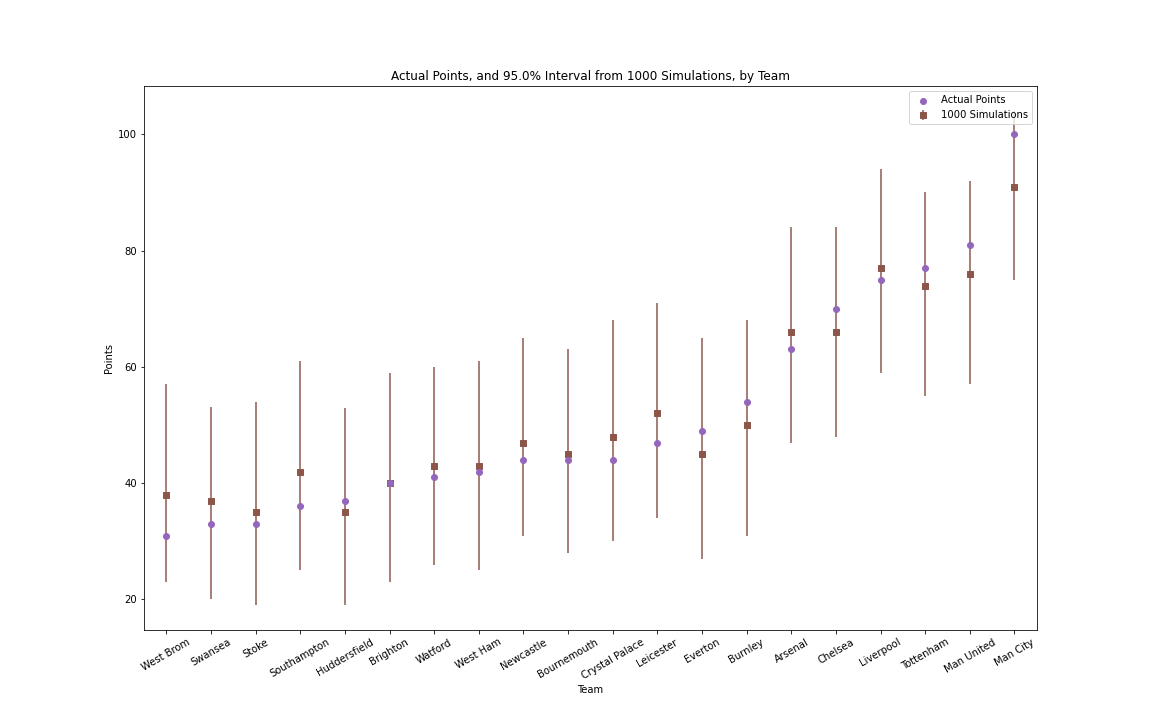
\includegraphics[width=40em]{Final_Report_Figures/simulation_vs_real_points_20000_4000_20.png}
\caption{Actual Points of the Season VS Median Points from the Simulated Seasons along with the 95\% CI for each team}
\label{fig:actual_simulation_points_barplot}
\end{figure*}

\begin{figure*}[!htb]
\centering
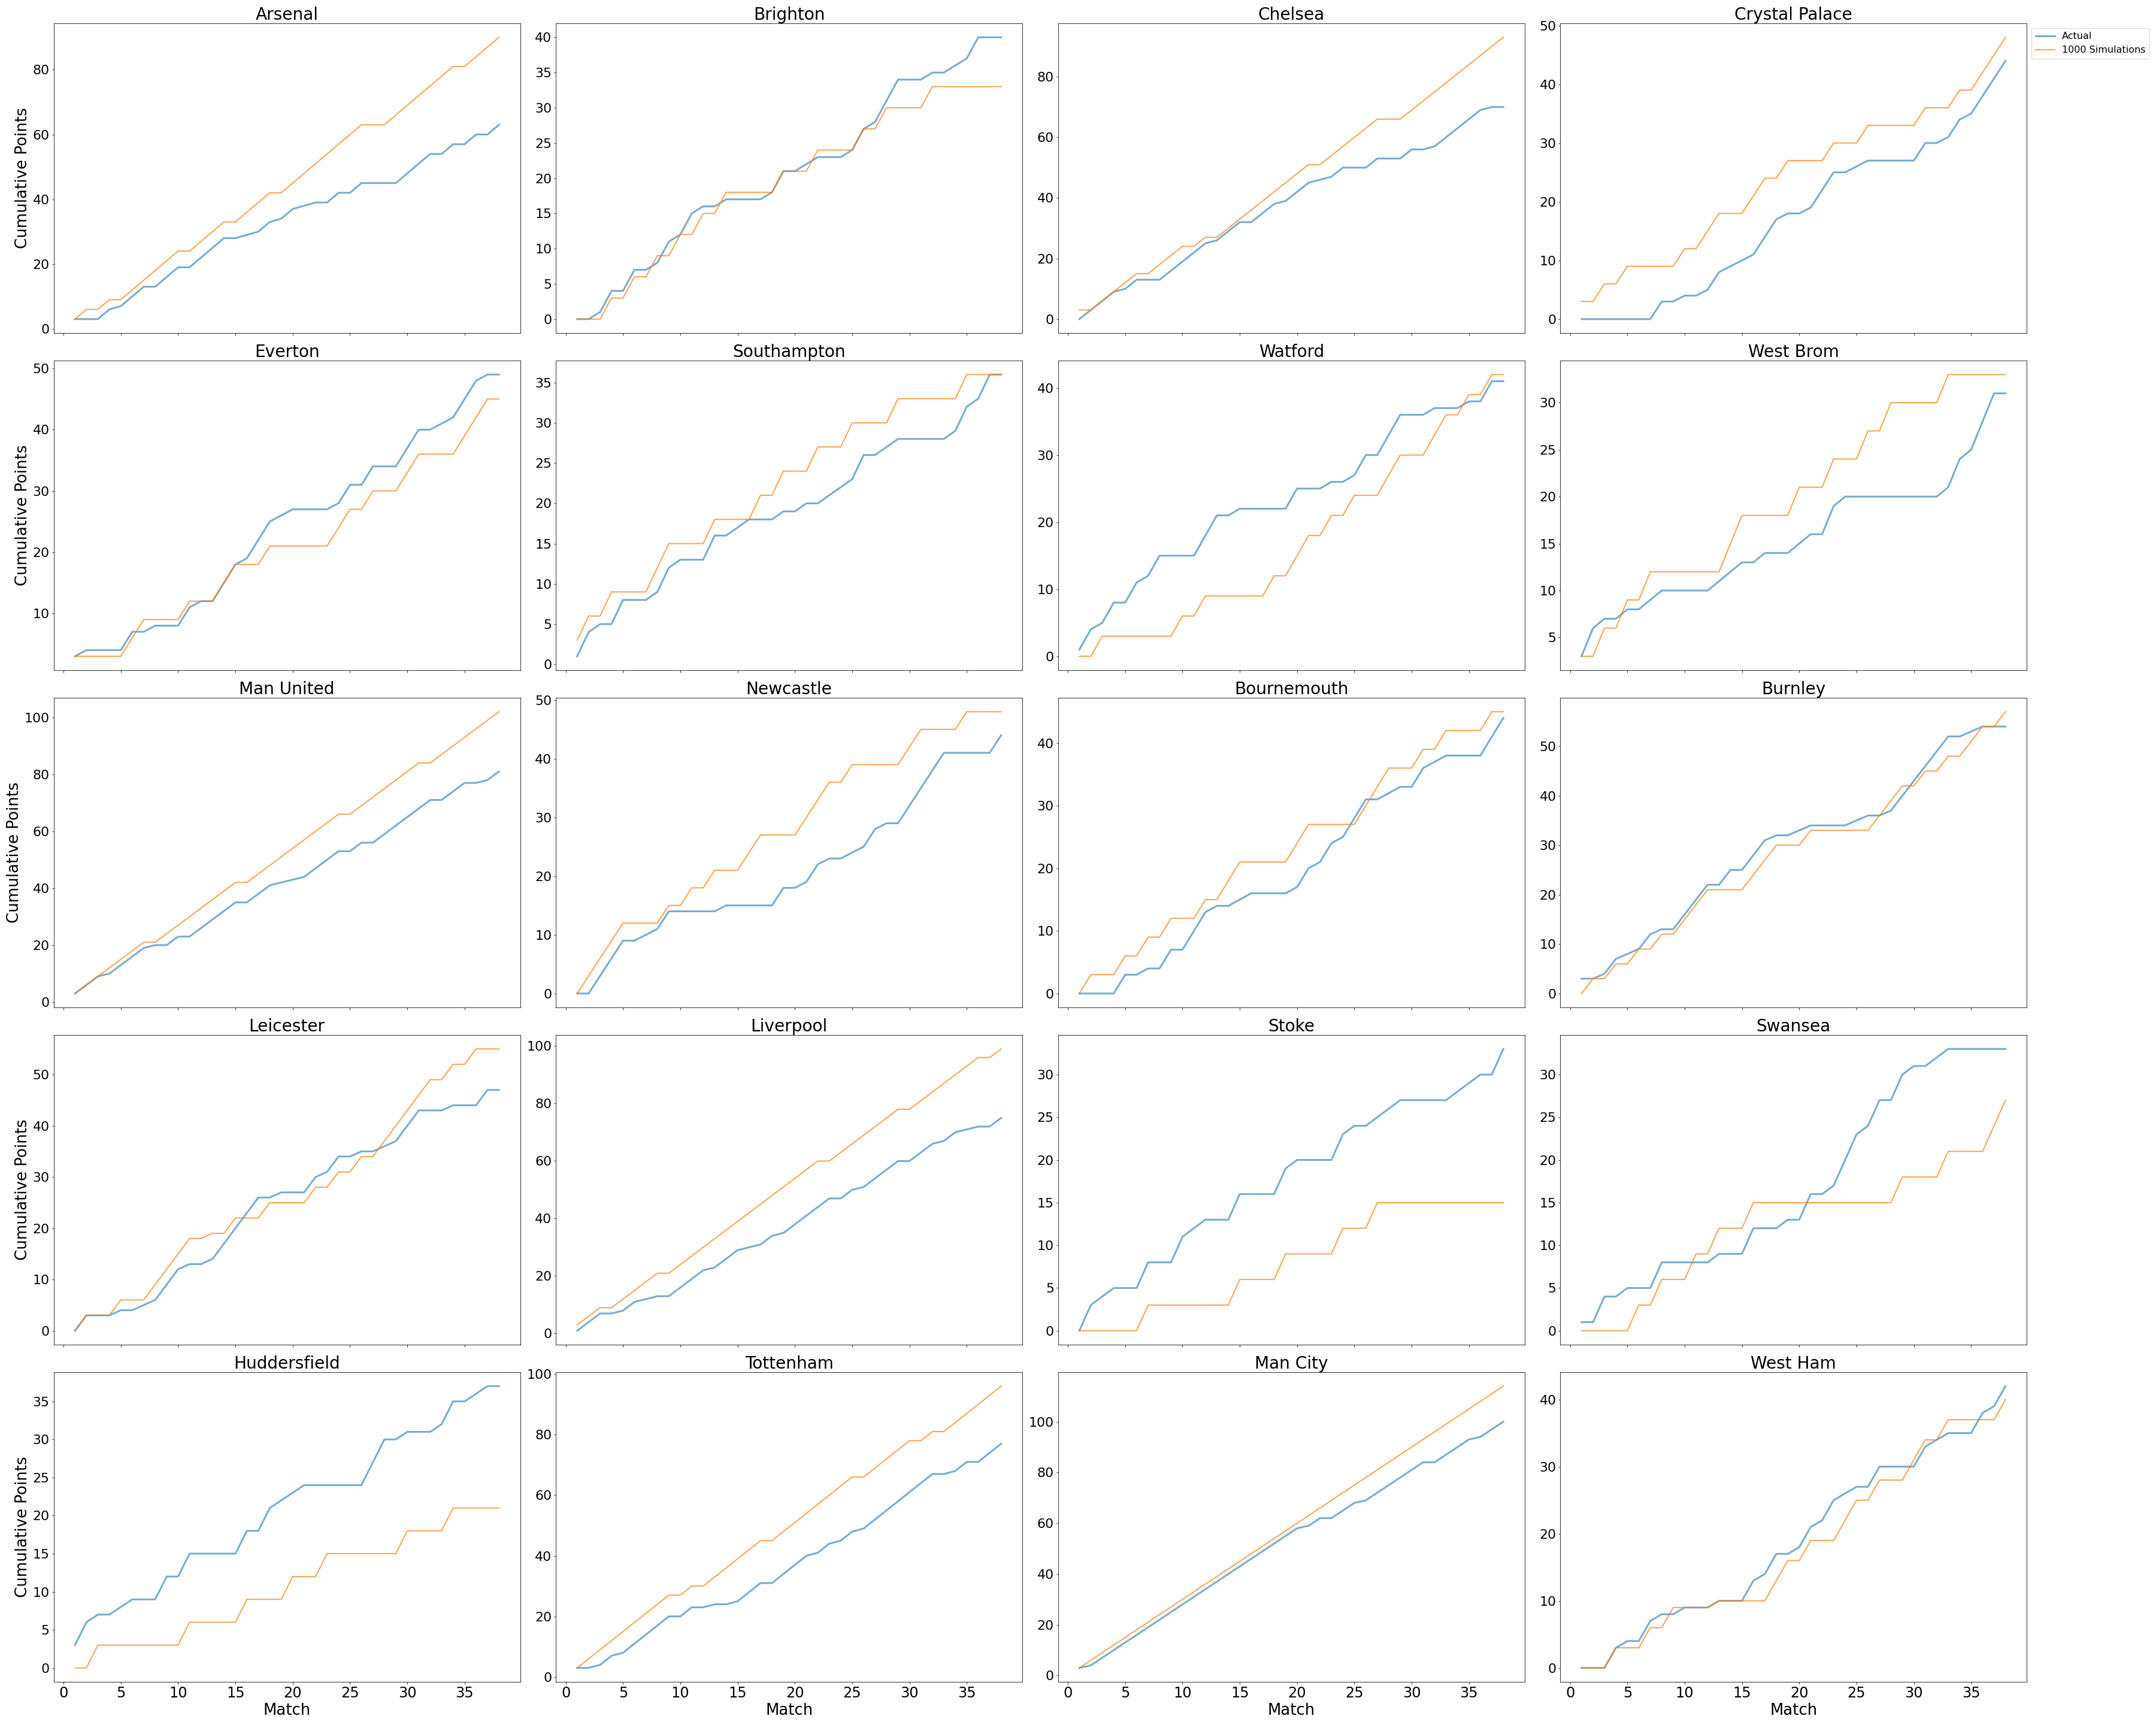
\includegraphics[width=40em]{Final_Report_Figures/Actual_vs_Prediction_Per_Match_Points_Team_4000_20.png}
\caption{Posterior predictive validation of the hierarchical model: the blue line represents the actual cumulative points acquired by each teams through the season, while the orange line represents the cumulative points  acquired by each teams through the season as predicted by the Bayesian Hierarchical Model}
\label{fig:actual_simulation_points_per_match}
\end{figure*}

% Please add the following required packages to your document preamble:
% \usepackage{multirow}
\begin{table}[!htb]
\centering
\begin{tabular}{c|ccc|ccc}
\multirow{2}{*}{Team} & \multicolumn{3}{c|}{Observed}          & \multicolumn{3}{c}{Bayesian Model}     \\
                      & Points & Goals Scored & Goals Conceded & Points & Goals Scored & Goals Conceded \\ \hline
Huddersfield          & 37     & 28           & 58             & 35     & 30           & 56             \\
Swansea               & 33     & 28           & 56             & 37     & 31           & 54             \\
West Brom             & 31     & 31           & 56             & 38     & 32           & 55             \\
Brighton              & 40     & 34           & 54             & 40     & 34           & 54             \\
Stoke                 & 33     & 35           & 68             & 35     & 36           & 66             \\
Burnley               & 54     & 36           & 39             & 50     & 37           & 39             \\
Southampton           & 36     & 37           & 56             & 42     & 38           & 54             \\
Newcastle             & 44     & 39           & 47             & 47     & 39           & 47             \\
Everton               & 49     & 44           & 58             & 45     & 44           & 56             \\
Watford               & 41     & 44           & 64             & 43     & 45           & 62             \\
Bournemouth           & 44     & 45           & 61             & 45     & 44           & 58             \\
Crystal Palace        & 44     & 45           & 55             & 48     & 46           & 54             \\
West Ham              & 42     & 48           & 68             & 43     & 47           & 65             \\
Leicester             & 47     & 56           & 60             & 52     & 55           & 58             \\
Chelsea               & 70     & 62           & 38             & 66     & 60           & 39             \\
Man United            & 81     & 68           & 28             & 76     & 66           & 30             \\
Arsenal               & 63     & 74           & 51             & 66     & 72           & 50             \\
Tottenham             & 77     & 74           & 36             & 74     & 71           & 37             \\
Liverpool             & 75     & 84           & 38             & 77     & 80           & 38             \\
Man City              & 100    & 106          & 27             & 91     & 101          & 30        
\end{tabular}
\caption{\label{tab:observed_bayesian_model_goals_points}Posterior Model Predictions of the Points and Scores against Observed Values}
\end{table}

\section{Conclusion}
The designed Bayesian Hierarchical Model successfully simulated and predicted results and statistics of individual matches in a season. The model validated the fact that there is an undue advantage which teams enjoy consistently while playing at home. Our model also incorporated multiple indirect features and engineered features to account for the perpetual performance of a team through the season. Finally, with such large variance in the performance of the teams, particularly with the top and bottom few, we detected a consistent issue of overshrinkage for both prediction of the points and the goals scored/conceded. This overshrinkage issue can be addressed by utilising mixture model prior instead of a flat distribution prior to better capture the wide difference in the teams’ attack and defense effects. We also hope to extend this model to calculate RPS score that is used by the betting organisations to guess match results.


\medskip

\printbibliography

\section{Supplement}

Below, figures \ref{fig:actual_simulation_goals_for_barplot} and \ref{fig:actual_simulation_goals_against_barplot} additional figures for comparing observed and simulated goals scored and conceded by each team.

\begin{figure*}[!htb]
\centering
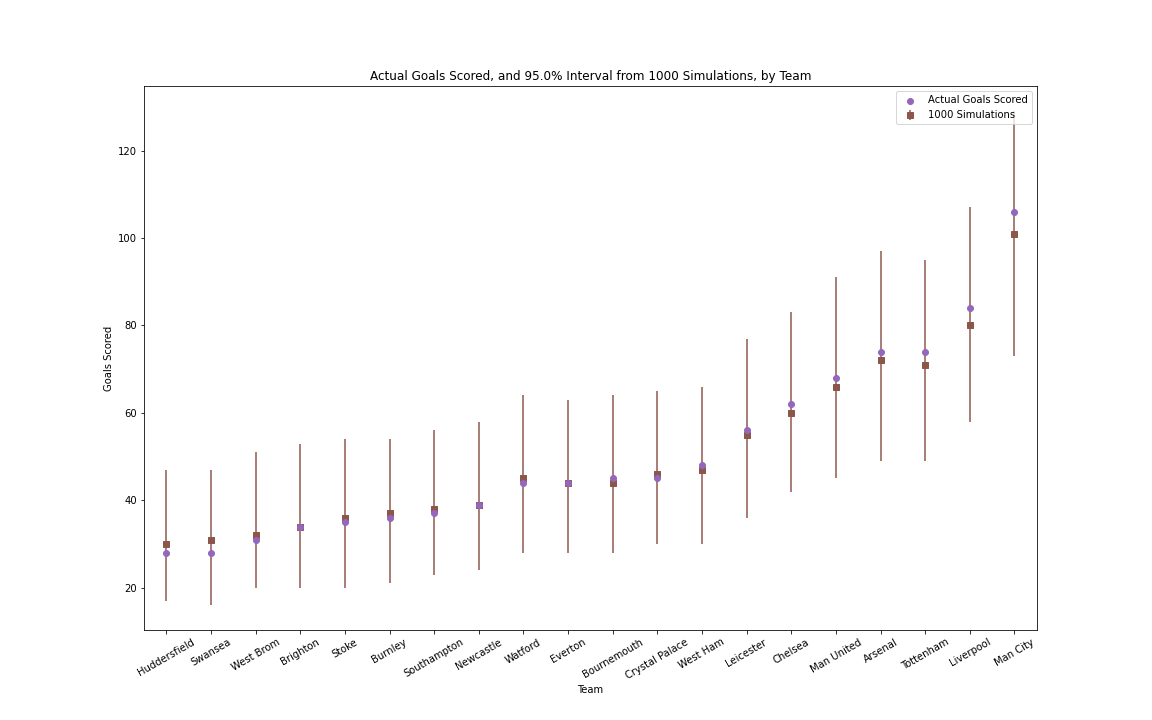
\includegraphics[width=40em]{Final_Report_Figures/simulation_vs_real_goals_for_20000_4000_20.png}
\caption{Actual Goals Scored of the Season VS Median Goals Scored from the Simulated Seasons along with the 95\% CI for each team}
\label{fig:actual_simulation_goals_for_barplot}
\end{figure*}

\begin{figure*}[!htb]
\centering
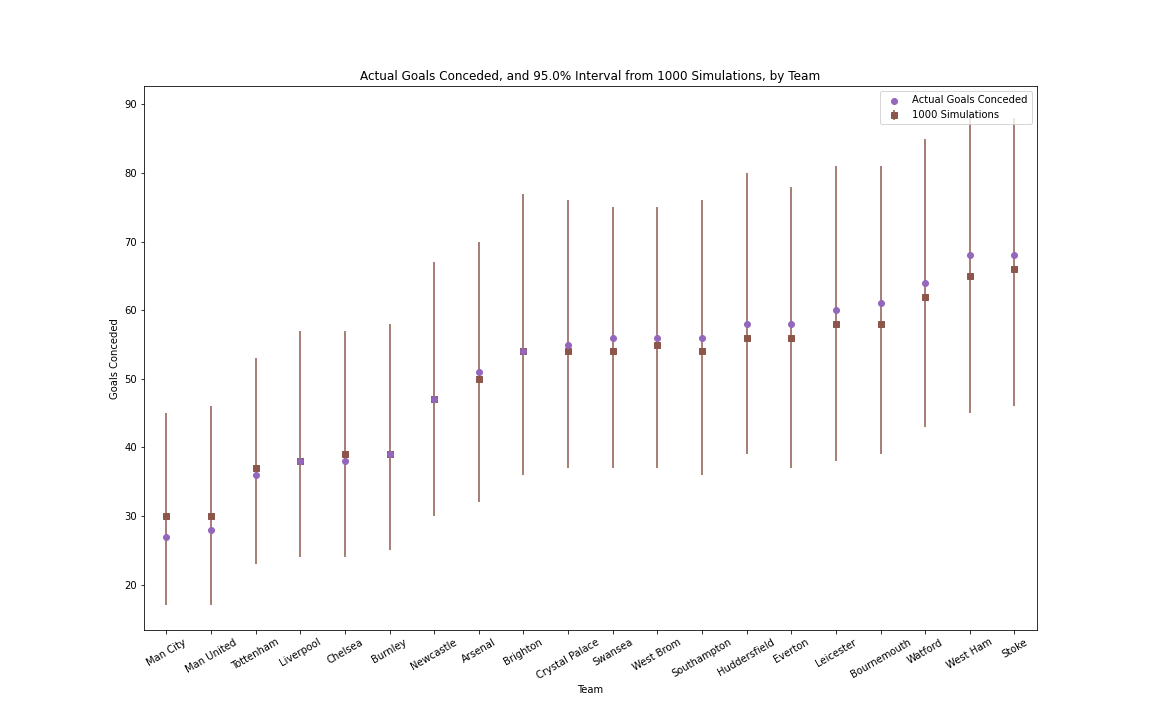
\includegraphics[width=40em]{Final_Report_Figures/simulation_vs_real_goals_against_20000_4000_20.png}
\caption{Actual Goals Conceded of the Season VS Median Goals Conceded from the Simulated Seasons along with the 95\% CI for each team}
\label{fig:actual_simulation_goals_against_barplot}
\end{figure*}
\end{document}
